%% ****** Start of file aiptemplate.tex ****** %
%%
%%   This file is part of the files in the distribution of AIP substyles for REVTeX4.
%%   Version 4.1 of 9 October 2009.
%%
%
% This is a template for producing documents for use with
% the REVTEX 4.1 document class and the AIP substyles.
%
% Copy this file to another name and then work on that file.
% That way, you always have this original template file to use.

% \documentclass[aip,pof,reprint]{revtex4-1}
% %\documentclass[aip,graphicx]{revtex4-1}
% %\documentclass[aip,reprint]{revtex4-1}
%
% \usepackage{graphicx}
% \usepackage[paperwidth=210mm,
%             paperheight=297mm,
%             centering,
%             hmargin=2cm,
%             vmargin=2.5cm]{geometry}
% \usepackage[colorlinks=true,
%             linkcolor=blue,
%             urlcolor=blue,
%             citecolor=blue]{hyperref}
% \graphicspath{{../Pyfig/to_convert/}}
% \usepackage{color}  % Probably not required, and was used for revisions
% \draft % marks overfull lines with a black rule on the right

% \begin{document}

% Use the \preprint command to place your local institutional report number
% on the title page in preprint mode.
% Multiple \preprint commands are allowed.
%\preprint{}

% \title{A two-dimensional toy model for geophysical turbulence} %Title of paper

% repeat the \author .. \affiliation  etc. as needed
% \email, \thanks, \homepage, \altaffiliation all apply to the current author.
% Explanatory text should go in the []'s,
% actual e-mail address or url should go in the {}'s for \email and \homepage.
% Please use the appropriate macro for the type of information

% \affiliation command applies to all authors since the last \affiliation command.
% The \affiliation command should follow the other information.

\author{Erik Lindborg}
%\email[]{Your e-mail address}
%\homepage[]{Your web page}
%\thanks{}
%\altaffiliation{}
\affiliation{Department of Mechanics, Osquars Backe 18, Royal Institute of Technology, Stockholm, Sweden}
\author{Ashwin Vishnu Mohanan}
%\email[]{Your e-mail address}
%\homepage[]{Your web page}
%\thanks{}
%\altaffiliation{}
% \affiliation{Department of Mechanics, Osquars Backe 18, Royal Institute of Technology, Stockholm, Sweden}

% Collaboration name, if desired (requires use of superscriptaddress option in \documentclass).
% \noaffiliation is required (may also be used with the \author command).
%\collaboration{}
%\noaffiliation

% \date{\today}
%
% \begin{abstract}
% A toy model for large scale geophysical turbulence is constructed by making two modifications of the shallow water model. Unlike the shallow water model the toy model has a quadratic expression for total energy, which is the sum of Available Potential Energy (APE) and Kinetic Energy (KE). More importantly, in contrast to the shallow water model the toy model does not produce any shocks. Three numerical simulations with different forcing are presented and compared with the simulation of a full General Circulation Model (GCM).  The energy which is injected cascades in a similar way as  in the GCM.
% First, some of the energy is converted from APE to KE at large scales.  The wave field is then undergoing a forward energy cascade displaying shallow spectra, close to $ k^{-5/3} $, for both APE and KE,  {while the vortical field
% either displays a $ k^{-3} $-spectrum or a more shallow spectrum, close to $ k^{-5/3} $, depending on the forcing. }
% In a simulation with medium forcing wave number, some of the energy which is converted from APE to KE is undergoing an inverse energy cascade which is produced by nonlinear interactions only involving the rotational component of the velocity field.  The inverse energy cascade builds up a vortical field at larger scales than the forcing scale. At these scales coherent vortices emerge with a strong dominance of anticyclonic vortices. The relevance of the simulation results to the dynamics of the atmosphere is discussed as is possible continuations of the investigation.
% \end{abstract}
%
% \pacs{}% insert suggested PACS numbers in braces on next line
%
% \maketitle %\maketitle must follow title, authors, abstract and \pacs

% Body of paper goes here. Use proper sectioning commands.
% References should be done using the \cite, \ref, and \label commands
\section{Introduction}

Large scale geophysical flows are often mentioned as possible applications in the context of two-dimensional (2D) turbulence whose fundamental features were first predicted in the seminal paper  by \citet{Kraichnan1967}, which this Focus Issue is commemorating.
\citet{Gage:1979} and \citet{Lilly:1983} suggested that the $ k^{-5/3} $ energy spectrum at atmospheric mesoscales, that are wave lengths from a few km up to five hundred km, measured by aircraft \citep{Nastrom-Gage:1985, Lindborg1999}, is produced by an inverse energy cascade of similar type as described by \citet{Kraichnan1967}, a  hypothesis which recently was revived by \citet{Xia2011}.
In the introduction of their excellent review article on 2D turbulence \citet{Boffetta2012} write that "large-scale motions in the atmosphere and oceans are described, to first approximation, as 2D turbulent fluids". There are almost countless examples of articles on 2D turbulence in which large scale geophysical flows are mentioned as possible applications.
However, the two-dimensional Navier-Stokes equations is  a very crude model for geophysical turbulence. Fundamental features of geophysical flows such as inertia-gravity waves are absent. Moreover, the inverse energy cascade of two-dimensional turbulence is far from telling the whole story  about energy exchanges between different scales of motion in the atmosphere. In Fig.~\ref{Flux} we have reproduced  a plot from \citet{Augier-Lindborg:2013} showing spectral energy fluxes calculated in the framework of spherical harmonics, $ Y_l^m $, from a General Circulation Model (GCM) called AFES \citep{Hamilton-Takahashi-Ohfuchi:2008}.
Using these base functions the spectral energy flux can be calculated from solutions to the primitive equations \citep{Vallis:book} on a sphere as a function of wave number $ l $, after summation over wave number $ m $, in a corresponding way as the spectral energy flux can be calculated in Fourier space from solutions of Navier-Stokes equations on a plane.
As shown by  \citet{Augier-Lindborg:2013} the flux can be calculated in a consistent way at each pressure level from a full  GCM. In the figure  we see spectral energy fluxes measured in $ W/m^2 $, integrated over all 24 levels of the model. In contrast to the case of  two-dimensional Navier-Stokes turbulence, the total spectral energy flux, $ \Pi (l) $  (black curve), of the primitive equations is the sum of the fluxes of two different forms of energy, the Kinetic Energy (KE) flux, $ \Pi_K(l) $, (red solid curve) and the flux, $ \Pi_A(l) $, of Available Potential Energy (APE) (blue curve). As shown by \citet{Lorenz:1955}, under certain approximations APE is quadratic in potential temperature and the sum of KE and APE is conserved by the primitive equations. For readers not familiar with Geophyscial Fluid Dynamics, potential temperature is the temperature a fluid element would have in case it would be adiabatically displaced to a reference pressure level.
In Fig.~\ref{Flux}, the fast increase of $ \Pi_A $  at  $ l \in [1, 3] $ means that  APE is forced at planetary scales of motions. The decrease of $ \Pi_A $ at $ l \in [8, 30] $ is matched by a corresponding increase of $ \Pi_K $. In this wave number range APE is converted into KE by baroclinic instability \citep{Vallis:book} which is the mechanism producing large scale weather systems.  The green curve, $ C_{cum}(l) $,  is the cumulative spectral conversion from APE to KE. A decrease of $ C_{cum}(l) $ in a certain wave number range corresponds to the amount of energy which is converted from APE to KE in that range.

\begin{figure}[h]
\centerline{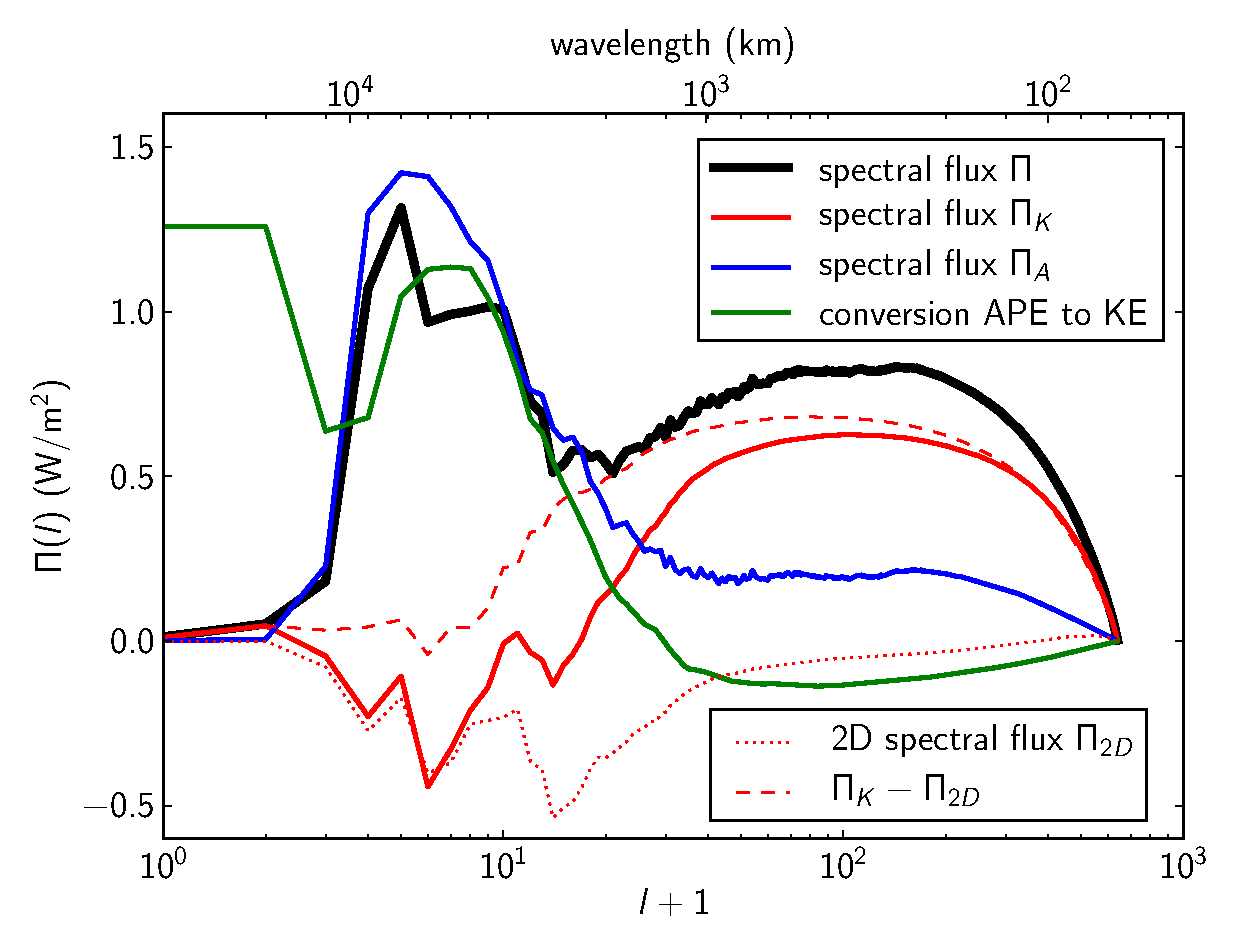
\includegraphics[angle=0,width=8cm]{./fig1.eps}}
 \caption{Spectral energy fluxes as functions of spherical harmonic wave number $ l $, calculated from the AFES GCM. The red solid curve is the KE flux, the blue curve is the APE flux, the black curve is the sum of KE and APE fluxes and the green curve is the accumulated APE-KE conversion. The dotted red curve is the 2D KE flux, calculated only from the rotational part of the velocity field, while the dashed curve is the difference between the total and the 2D KE flux.
Reprinted
with permission from P. Augier \& E. Lindborg,
"A new formulation of the spectral energy budget of the atmosphere, with application to two high-resolution general circulation models",
J. Atmos. Sci. \textbf{70}, 2293--2308 (2013).
Copyright 2013 American Meterological Society.
}
 \label{Flux}
 \end{figure}


Some of the energy which is converted from APE to KE goes into an inverse energy cascade, as is clear from the fact that $ \Pi_K < 0 $ for $ l < 10 $. This inverse cascade is the energy source of the large scale circulation of the atmosphere. According to the model, approximately $ 0.5 \; W/m^2 $ is going into the inverse energy cascade. This cascade is produced by nonlinear interactions of the same type as is giving rise to the inverse energy cascade of the two-dimensional incompressible Navier-Stokes equations. To explain this further we make a Helmholtz decomposition of the horizontal velocity field,
\begin{equation}
{\bf u} = \bf{u}_r + \bf{u}_d \, ,
\end{equation}
where
\begin{equation}  {\bf u}_r  = -\nabla \times ( {\bf e_z} \Psi) \, , \end{equation}
is the rotational component and
\begin{equation}  \bf {u}_d = \nabla \chi  \, , \end{equation}
is the divergent component of the velocity field,  $ \Psi  $ is the stream function,  $ \chi $ is the velocity potential and $ {\bf e}_z $ is the vertical unit vector.  In this paper we will not go into the problem of uniqueness of the Helmholtz decomposition, but assume that it can be carried out in an unambiguous way, as is the case  with a flow field on a sphere or on a square domain if we apply periodic boundary conditions.  The KE flux in Fig.~\ref{Flux} is decomposed into two parts,  the 2D-part (dotted red curve) that contains contributions from nonlinear interactions only involving $ {\bf u}_r $ and the remaining part (red dashed curve) that contains contributions from interactions also involving $ {\bf u}_d $. As seen from the figure, it is the 2D-part that produces the inverse energy cascade, while the other part is actually producing a forward energy cascade of approximately the same magnitude.
In the model, this forward energy cascade is giving rise to a KE spectrum with an approximate  $ -5/3 $ power law in the spherical harmonic wave number $ l $.    The spectral flux of APE is also positive in the same range and the APE spectrum also shows an approximate  $-5/3 $ power law dependence. When velocity and temperature are decomposed into Fourier modes with wave number $ k $, both KE- and APE-spectra exhibit an extended $ k^{-5/3} $ range at atmospheric mesoscales as  demonstrated by \citet{Nastrom-Gage:1985}.  As mentioned previously, \citet{Gage:1979} and \citet{Lilly:1983}    suggested that the $ k^{-5/3} $ mesoscale range is produced by an inverse or upscale energy cascade of similar type as in 2D turbulence. However, there is an emerging consensus that the mesoscale spectrum is associated with a downscale energy cascade of Kolmogorov type, as first suggested by \citet{Dewan:1979}. There is still a lively debate whether the three-dimensional motions behind this cascade should be characterised as weakly nonlinear waves \citep{Callies-Ferrari-Buhler:2014, Waite-Snyder:2013}, or as turbulence \citep{Lindborg:2015}. In this paper we will not go into this debate but take a completely different approach.



Theories that are trying to explain the mesoscale $ k^{-5/3} $ spectrum predict that the three-dimensional structures behind the forward energy cascade are very thin and elongated. \citet{Lindborg2006} and
\citet{Waite-Bartello:2004}  emphasise that  it is necessary to have a vertical resolution which is finer than the buoyancy scale, $ \l_b= u/N $, in order to simulate the downscale energy cascade. Here, $ u $ is a characteristic horizontal velocity and $ N $ is the Brunt-V\"sisal\"a frequency. In the upper troposphere and the lower stratosphere $ l_b $ can be estimated to be of the order of one km at most.  According to the hypothesis  of \citet{Callies-Buhler-Ferrari:2016} the mesoscale energy spectrum is built up by inertia-gravity waves with frequencies very close to the inertial frequency $ f $. The ratio between the vertical and the horizontal wave length of such waves is extremely small. With a horizontal wave length $ \lambda_{h} \sim 100 $ km, the corresponding vertical wave length would be a few hundred meters. Despite the prediction of these theories that a very fine resolution would be needed in order to simulate the downscale mesoscale energy cascade it is a fact that GCMs such as the AFES-model and the MPAS-model \citep{Skamarock-Park-Klemp-Snyder:2014} are able to do this although they lack the required vertical resolution. This fact has lead us to the following questions: What is the minimum number of levels that are needed in order to simulate the mesoscale downscale energy cascade? Is it even possible to do this with a single level model, in other words with a two-dimensional model? It is the aim of the present paper to construct such a model.

\section{Development of the toy model}
It is clear from the previous discussion that  a  two-dimensional model that is able to produce both an inverse and a forward energy  cascade must allow for a divergent component of the two-dimensional velocity field.
To mimic geophysical turbulence the model should also contain a scalar playing the role of potential temperature. Preferably, total energy should be the sum of KE and APE, KE should be quadratic in the velocity, APE should be quadratic in the scalar and the equations for KE and APE should contain an exchange term allowing for a velocity field to develop if the model is forced in the scalar field.

We first consider the shallow water model \citep{Vallis:book} and discuss why this  is not a fully satisfactory model for Geophysical Turbulence, despite the fact that it has several attractive features. The shallow water set of equations can be written as
\begin{eqnarray} \label{Velocity}
\frac{\partial {\bf u}} {\partial t} + {\bf u} \cdot \nabla {\bf u} +  f {\bf e}_z \times {\bf u} = -c^2 \nabla \eta \, , \\ \label {Eta}
\frac{\partial \eta}{\partial t}
+ {\bf u} \cdot \nabla \eta   = - (1+\eta) \nabla \cdot {\bf u} \, ,
\end{eqnarray}
where $ \eta \ll 1 $ is the non-dimensional surface displacement of a shallow water layer with unity depth, $ c = \sqrt{gD} $ is the phase velocity of surface gravity waves, $ g $ being the acceleration due to gravity and $ D $ the dimensional depth of the layer, and $ f  $ is the Coriolis parameter. In this paper we will not consider the case with differential rotation, that is a $ \beta $-plane on which $ f = f_{0} + \beta y $, where  $ y $ is the coordinate in the meridional direction, but restrict the study to an $ f $-plane on which $ f $ is constant.
The shallow water model conserves the sum of kinetic energy and enthalpy, defined as
\begin{eqnarray}
E_K = (1+\eta) \frac{{\bf u} \cdot {\bf u}}{2} \, , \\  \label{potential}
H = c^{2} \left (\alpha + \beta \eta  + \frac{(1+\eta)^2 }{2} \right) \, ,
\end{eqnarray}
where $ \alpha $ and $ \beta $ are two arbitrary constants.
We define APE by putting $  \alpha = -1/2 $ and $ \beta = - 1 $  in the expression for $ H $, that is
 \begin{equation}
E_{A} = \frac{c^2  \eta^{2} }{2} \, .
\end{equation}
The equations for $ E_K $ and $ E_A $ are
\begin{eqnarray} \label{KE}
\frac{\partial{E_K}} {\partial t} + \nabla \cdot ({\bf u}E_K) = -{\bf u} \cdot \nabla \left (\frac{c^2(1+\eta)^2}{2} \right ) \, , \\
\frac{\partial{E_A}} {\partial t} + \nabla \cdot({\bf u} (2E_A + \eta c^{2})) = {\bf u} \cdot \nabla \left (\frac{c^2(1+\eta)^2}{2} \right ) \, .
\end{eqnarray}
The shallow water model also has another interesting property. Potential vorticity, defined as
\begin{equation} \label{PV}
Q = \frac{f +\zeta }{1+\eta} \, ,
\end{equation}
where $ \zeta =  \nabla^{2} \Psi $ is the vorticity, is a materially conserved quantity.
This property is extensively explored in text books on Geophysical Fluid Dynamics (e.g., \citet{Vallis:book}) to illustrate interesting features of geophysical flows. { However, as discussed by \citet{Warn1986}  conservation of $ Q $ is not a property that is very useful from the point of view of turbulence theory, since potential enstrophy, defined as the square of $ Q $,  is not a quadratic quantity in the flow quantities.  As shown by \citet{Warn1986} it is only in the limit when $ Q $ becomes a linear quantity that
 conservation of $ Q $ will not lead to any constraints on cascade directions. }  In the limit of strong rotation, or the Quasi Geostrophic (QG) limit \citep{Charney1971}, potential enstrophy becomes a quadratic quantity and so does total energy.  In this limit,  shallow water turbulence is very similar to 2D turbulence, since there are two related quadratic invariants and $ {\bf u}_d $ is zero. This limit will be discussed below.

At first glance the shallow water model seems to be a promising candidate for a two-dimensional model of geophysical turbulence that might be capable of reproducing the same type of energy exchanges and energy cascades as displayed in Fig.~\ref{Flux}.
The velocity field has both a rotational and a divergent component. Moreover, the model contains a scalar playing a similar role as potential temperature, APE is quadratic in the scalar,
the sum of KE and APE is conserved and there is a term associated with exchange between the two forms of energy.  From the point of view of turbulence theory it is a drawback that kinetic energy is not a quadratic quantity, but since it must be assumed that $ \eta \ll 1 $, kinetic energy is approximately quadratic.

The shallow water model has been studied from the point of view of turbulence theory by several investigators \citep{FargeSadourny1989, YuanHamilton1994, Dritschel2001}.
As shown in these studies shallow water turbulence can be decomposed into a vortical field and a wave field. The vortical field shares some properties with two-dimensional Navier-Stokes incompressible turbulence while the  wave field undergoes a forward energy cascade. However, strong discontinuities or shocks develop in the wave field, as observed by \citet{SpallMcWilliams1992}.
In a companion paper \citep{AugierMohananLindborg2017} we show that the forward energy cascade of the shallow water wave field is dominated by such shocks,
giving rise to a $ k^{-2} $-spectrum, which is  characteristic of shock dominated turbulence \citep{Kuznetsov2004}, such as turbulence arising from Burger's equation  \citep{BouchaudMezardParisi1995}.  It is obvious that this type of turbulence has little to do with mesoscale dynamics in the atmosphere where no shocks are observed. \citet{Buhler1998} has shown that the shallow water model can be modified in such a way that shocks are avoided. This is accomplished by replacing the term  $ -c^{2} \nabla \eta $ on the right hand side of equation (\ref{Velocity}) by  $ -c^{2}(1+\eta)^{-3} \nabla \eta $. However, the  expression for enthalpy will in this case take the form $ H = c^2( \alpha \eta + \beta \eta+ (1+\eta)^{-1}/2) $, and there is no way to define APE such that it becomes quadratic in $ \eta $.
We will instead introduce two other modifications of the shallow water model that will remove the shocks and also give an expression for total energy which is quadratic. The first modification we introduce is to replace the term
$ -(1+\eta) \nabla \cdot  {\bf u} $ on the right hand side of (\ref{Eta}) by $ -\nabla \cdot {\bf u} $. This modification can be motivated from the assumption $ \eta \ll 1 $, which is already inherent in the shallow water model.
{ Equation (\ref{Eta}) of the shallow water model is derived from mass conservation. If this interpretation also is made of the modified equation,  mass conservation is not perfectly fulfilled, but only to the extent that $ \eta $ is small.}  The second modification is motivated by introducing the assumption that the large scale motions are dominated by the rotational component of the velocity field.  We define the fields in square domain $
[0 \; 2\pi]^2 $, apply periodic boundary conditions and denote the 2D Fourier transform of a quantity by putting a hat on it. We decompose the rotational and divergent velocity fields into large and small scale fields as
\begin{eqnarray}
{\bf u}_r = {\bf u}_r^{l} + {\bf u}_r^{s} \, , \;\;\;\;
{\bf u}_r^{l} = \sum_{k < k_{d}} -{\mbox{i}} {\bf k} \times {\bf e}_z \widehat{\psi}  \exp({\mbox{i}}{\bf k}\cdot {\bf r}) \, , \\
{\bf u}_d = {\bf u}_d^{l} + {\bf u}_d^{s} \, , \;\;\;\;
{\bf u}_d^{l} = \sum_{k < k_{d}} {\mbox{i}} {\bf k} \widehat{\chi}  \exp({\mbox{i}}{\bf k}\cdot {\bf r}) \, ,
\end{eqnarray}
where $ k = |{\bf k} | $ and $ k_d = f/c $ is the wave number corresponding to the deformation radius $ r_d = c/f $.  We also decompose the vorticity, $ \zeta = \nabla^{2} \psi $, and the divergence , $ d = \nabla^2 \chi $, in the same way,
\begin{eqnarray}
\zeta = \zeta^l + \zeta^s \, , \;\;\;\;  \zeta ^{l} = \sum_{k < k_{d}} -k^2 \widehat{\Psi} \exp({\mbox{i}}{\bf k}\cdot {\bf r}) \, , \\
d = d^l + d^s \, , \;\;\;\;  d ^{l} = \sum_{k < k_{d}} -k^2 \widehat{\chi} \exp({\mbox{i}}{\bf k}\cdot {\bf r}) \, ,
\end{eqnarray}
and make the following assumptions
\begin{eqnarray} \label{LargeAssumption}
 | {\bf u}_r^{l} | \gg  | {\bf u}_r ^{s} | \, , \;\; | {\bf u}_d^{l} | \gg  | {\bf u}_d ^{s} | \, , \;\;
 | {\bf u}_r^{l} | \gg | {\bf u}_d^{l} | \, , \\  \label{SmallAssumption}
 | \zeta^{l} | \ll | \zeta^{s} | \, , \;\;   | d^{l} | \ll | d^{s} | \, , \;\;
 | \zeta^{s} | \sim | d^{s} | \, .
\end{eqnarray}
Indeed, these assumptions are consistent with atmospheric dynamics, where the velocity field is dominated by large scale rotational motions, while the vorticity and divergence fields are dominated by contributions from the high wave number end of the $ k^{-5/3} $-spectrum range and are of the same order of magnitude
\citep{Lindborg:2015}.
Under the assumption (\ref{LargeAssumption})   we can approximate the advective operator $ {\bf u} \cdot \nabla $ by
$ {\bf u}_r \cdot \nabla $. This is the same type of approximation that is made in the QG approximation \citep{Charney1971}.
However, there is an important difference. The assumption (\ref{SmallAssumption}) does not permit us to neglect the derivatives of $ {\bf u}_d $ that arise when the advective operator is acting on the velocity field.
Introducing these modifications in the shallow water equations the toy model equations can be written as
\begin{eqnarray} \label{V2}
\frac{\partial {\bf u}} {\partial t} + {\bf u}_r \cdot \nabla {\bf u} + f {\bf e}_z \times {\bf u} = -c \nabla \theta + (-1)^{p+1} \nu_p \nabla^{2p} {\bf u} , \\ \label{Theta}
\frac{\partial \theta}{\partial t}
+ {\bf u}_r \cdot \nabla \theta   = -  c\nabla \cdot {\bf u} + (-1)^{p+1} \nu_p \nabla^{2p} {\theta}\, ,
\end{eqnarray}
where we have introduced the notation $ \theta = c \eta $ for the scalar and also added diffusion terms.
Although it is very difficult to prove, it is quite easily argued that no shocks will arise from equations (\ref{V2}) and (\ref{Theta}), even in the absence of diffusion terms.  Locally, shock formation can be viewed as a one-dimensional process in which a gradient along a specific direction, say the $ x $-direction,  is amplified through nonlinear interactions. In the case  when $ {\bf u} = u {\bf e}_x + v {\bf e}_y $  and $ \theta $ are only functions of $ x $, we find that $ {\bf u}_r = v {\bf e}_y $ and the nonlinear terms in (\ref{V2}) and (\ref{Theta}) are zero. Therefore, no shocks will form in the one-dimensional case and it is therefore arguable that no shocks will be formed in the general two-dimensional case.

The toy model equations can be expressed as three coupled equations for $ \Psi $, $ \chi $ and $ \theta $. Unfortunately, we have found no elegant way in which they can be expressed in vector notation, why we write them as
\begin{align} \label{PsiEq}
&\frac{\partial{\Psi_{ii}}}{\partial t} +\epsilon_{ijk}e_k \Psi_i \Psi_{jll} + \Psi_{ii} \chi_{jj} - \Psi_{ij} \chi_{ij} = -f \chi_{ii} + (-1)^{p+1} \nu_p \nabla^{2p} \Psi_{ii} \, , \\ \label{ChiEq}
&\frac{\partial{\chi_{ii}}}{\partial t} +\epsilon_{ijk}e_k (\Psi_i \chi_{jll} -
\Psi_{jl} \chi_{il}) + \Psi_{ij} \Psi_{ij} - \Psi_{ii} \Psi_{jj} \nonumber\\
&\quad=  f \Psi_{ii} - c \theta_{ii} + (-1)^{p+1} \nu_p \nabla^{2p} \chi_{ii} \, , \\ \label{ThetaEq}
&\frac{\partial{\theta}}{\partial t} + \epsilon_{ijk}e_k \Psi_i \theta_{j} = - c \chi_{ii} + (-1)^{p+1} \nu_p \nabla^{2p} \theta \, ,
\end{align}
where $ e_k $ is the vertical unit vector expressed in three-dimensional Cartesian tensor notation,  subscript $ i $  has the same meaning as $ {\partial }/{\partial x_i }$ when used on $ \Psi $,  $ \chi $ or $ \theta $ and repeated indices means summation.


The toy model expression for  KE and APE are quadratic,   $ E_K = {\bf u}\cdot {\bf u}/2 $ and $ E_A = \theta^2/2 $.
In the absence of diffusion terms the equations for $ E_K $ and $ E_A $ can be written as
\begin{eqnarray} \label{EK}
\frac{\partial{E_K}} {\partial t} + \nabla \cdot ({\bf u}_rE_K+ c{\bf u}_r \theta) = - c \nabla \theta \cdot {\bf u}_d  \, , \\ \label{EA}
\frac{\partial{E_A}} {\partial t} + \nabla \cdot ({\bf u}_rE_A + c{\bf u}_d  \theta) =  c \nabla \theta \cdot {\bf u}_d \, .
\end{eqnarray}
 The term on the right hand side of  (\ref{EK}) is the same as the term on the right hand side of (\ref{EA}) apart from the sign. In other words, this term is conversion from APE to KE.
The potential vorticity, $ Q $,  as defined in (\ref{PV}), is not conserved by the toy model. This is the price that we have to pay in order to obtain a model that does not produce any shocks and has a quadratic expression for total energy. As we discussed above, since $ Q $ is not a linear quantity in the flow quantities conservation of $ Q $  is not a very interesting property of the shallow water model if we look at it strictly from the point of view of turbulence theory.
We are therefore willing to pay this price. Instead of studying $ Q $ we study  linear potential vorticity  \citep{Dritschel2001} defined as
\begin{equation} \label{Linear}
q = \zeta - \frac{f}{c}\theta .
\end{equation}
In the QG limit $ q $ is a materially conserved quantity in the shallow water model \citep{Vallis:book}. This is also the case in the toy model.
The equation for $ q $ is derived as a linear combination of  (\ref{PsiEq}) and (\ref{ThetaEq}),
\begin{equation}
\frac{\partial q }{\partial t} + {\bf u}_r \cdot \nabla q  =  \Psi_{ij} \chi_{ij} - \Psi_{ii} \chi_{jj} \, ,
\end{equation}
where we have excluded diffusion terms. A small parameter expansion of  the equations (\ref{PsiEq} - \ref{ThetaEq}) in the Rossby number \citep{Vallis:book} $ Ro $ gives that $ \chi \sim Ro \Psi $ and in the limit $ Ro \rightarrow 0 $, $ q $ will be a materially conserved quantity.


We define the KE and APE spectra as
\begin{eqnarray}
E_K(k) =\sum_{B(k)}  \frac{1}{2}  \widehat{\bf u} \cdot \widehat{\bf u}^{\star}  \, , \\
E_A(k) = \sum_{B(k)} \frac{1}{2} \widehat{\theta} \widehat{\theta}^{\star} \, ,
\end{eqnarray}
where $ ^{\star} $ denotes the complex conjugate and the summation is over
all $ k_x $ and $ k_y $ such that $ \sqrt{k_x^2+k_y^{2}} $ lies within the wavenumber band,  $ B(k) $,   centered at $ k $ and with unity width. The equation for the energy spectra can be written as
\begin{eqnarray}
\frac{\partial{E_K}(k)} {\partial t}  = T_K(k) + C (k) - \nu_p k^{2p} E_K(k) \, , \\
\frac{\partial{E_A}(k)} {\partial t}  = T_A(k) - C (k) - \nu_p k^{2p} E_A(k) \, ,
\end{eqnarray}
where
\begin{eqnarray}
T_{K}(k) = \sum_{B(k)} Im [  k_j \widehat{u_{rj} u_i} \widehat{u}_i ^{\star} ]  \, , \\
T_{A}(k)  = \sum_{B(k)} Im [ k_j \widehat{u_{rj} \theta} \widehat{\theta} ^{\star}] \, , \\
C (k) = \sum_{B(k)} Re[ c k^{2}\widehat{\theta} \widehat{\chi}^{\star}] \, .
\end{eqnarray}
are spectral transfer and conversion terms. The spectral flux of kinetic and potential energy are defined as
\begin{eqnarray}
\Pi_K(k) = \sum_{k^{\prime} = k}^{k_{m}} T_K(k^{\prime}) \, , \\
\Pi_A(k) = \sum_{k^{\prime} = k}^{k_{m}} T_A(k^{\prime}) \, ,
\end{eqnarray}
where $ k_{m} $ is the maximum wave number in the Fourier decomposition. The cumulative spectral conversion is defined as
\begin{equation} \label{Cum}
C_{cum} (k)  = \sum_{k^{\prime} = k}^{k_{m}} C (k^{\prime}) \, .
\end{equation}
Unlike the energy fluxes, $ C_{cum} $ does not go to zero in the limit $ k =0 $, but approaches the total mean conversion of APE to KE.
Potential enstrophy,  defined as $ q^2/2 $,  will be an inviscidly conserved quantity in the QG limit. Therefore, it may be interesting to study spectral transfer and spectral flux of potential enstrophy. We define these quantities as
\begin{eqnarray}
T_{q} =  \sum_{B(k)} Im [ k_j \widehat{u_{rj} q} \widehat{q}^{\star}]  \, , \\
\Pi_{q} = \sum_{k^{\prime} = k}^{k_{m}} T_{q} (k^{\prime}) \, .
\end{eqnarray}
 Following \citet{Bartello:1995} and \citet{Dritschel2001} we decompose the flow field into normal  modes which we define as the three normalised eigenmodes of the linear inviscid part of the system (\ref{PsiEq}-\ref{ThetaEq}) in Fourier space. These modes are
\begin{eqnarray}
\widehat{a}_{1} = \frac{k}{\sqrt{2} \omega} ( c \widehat{\theta} + f \widehat{\Psi} - {\mbox{i}} \omega \widehat{\chi} )  \\
\widehat{a}_{2} =  \frac{k}{\sqrt{2} \omega} ( c \widehat{\theta} - f \widehat{\Psi} + {\mbox{i}} \omega \widehat{\chi} ) \\
\widehat{b} =  \frac{1}{\omega} (c k^2 \widehat{\Psi}-f \widehat{\theta}   ) \\
\end{eqnarray}
where
\begin{equation} \label{Dispersion}
\omega =  \sqrt{f^2+k^2c^2}  \, .
\end{equation}
The modes $ \widehat{a}_{1} $ and $ \widehat{a}_{2} $ are associated with inertia-gravity waves with frequencies $ \pm \omega $.
The mode $ \widehat{b} $, on the other hand,  is associated with linear potential vorticity (\ref{Linear}).
We define the wave and the vortical energy spectra as
\begin{eqnarray}
E_{W}(k) = \sum_{B(k)} \frac{1}{2}(\widehat{a}_{1} \widehat{a}_{1}^{\star} + \widehat{a}_{2} \widehat{a}_{2}^{\star} ) \, , \\
E_{V}(k) =  \sum_{B(k)} \frac{1}{2} \widehat{b} \widehat{b} ^{\star} \, .
\end{eqnarray}
{ \noindent Following \citet{Deusebio-Vallgren-Lindborg:2013} the total energy transfer can be decomposed into four terms as
\begin{equation}
T_K(k) + T_A(k) = T_{VVV}(k) + T_{VVW}(k) + T_{VWW} + T_{WWW} \, ,
\end{equation}
where
$ T_{VVV} $ represents the contribution from triad interactions between three vortical modes, $ T_{VVW} $  two vortical modes and one wave mode,  $ T_{VWW} $ one vortical mode and two wave modes and $ T_{WWW} $ three wave modes.  It can be shown that each of these four  terms integrates to zero and  thus conserves energy. Accordingly, the total energy flux may  also be decomposed into four terms as
\begin{equation} \label{Decomposition}
\Pi_K(k) + \Pi_A(k) = \Pi_{VVV}(k)+ \Pi_{VVW}(k)+\Pi_{VWW}(k)+ \Pi_{WWW}(k) \, .
\end{equation} }
\noindent We are now in the possession of the tools that are needed in order to explore a numerical simulation of the toy model.

\section{Numerical simulations}
In this section we will present { three}  simulations of the toy model showing that it does not produce any shocks, unlike the shallow water model, and that it is capable of reproducing energy exchanges and cascades that are similar to what is displayed in Fig.~\ref{Flux}.  A more comprehensive numerical study will be presented in a future paper.

The equations (\ref{PsiEq}-\ref{ThetaEq}) are solved in a square domain  using a standard pseudo spectral method and a fourth order Runge-Kutta scheme, in which the time step is set by a CFL-condition guaranteeing both numerical stability and that fast gravity waves are resolved.   A random forcing is  injecting energy into the system at a rate $ P $, which is approximately equal to unity.
The forcing is white noice in time and restricted to a narrow range in Fourier space centered at wave number $ k_f $. Initially, the wave field is set to zero while the vortical field is initialised with a very low amplitude random noise at the forcing wave number to facilitate for the vortical field to build up.
The parameters $ f $ and $ c $ are specified in terms of the Rossby and the Froude numbers defined as
\begin{eqnarray}
Ro = \frac{P^{1/3} k_f^{2/3}}{f} \, , \\
Fr = \frac{P^{1/3}}{k_f^{1/3} c}  \, .
\end{eqnarray}
We use resolution $ n = 1920 $ in both directions and dealiasing with truncation in Fourier modes  lying outside the square $ | k_y | <  k_{max} $,  $ | k_x | < k_{max} $,  where $ k_{max} = 4n/9 $.
We chose  $ p = 4 $ as the order of the diffusion terms in (\ref{PsiEq}-\ref{ThetaEq}).  { Assuming that the simulations will reach a quasi stationary state in which $ \epsilon \approx P $, where $ \epsilon $ is the dissipation, $ \nu_4 $  is set so that $ k_{diss}/k_{max} \approx 1$, where $ k_{diss} = \epsilon^{1/3}/\nu_4^{3/22} $. With this choice of $ \nu_4 $ it was found that the peak of the dissipation spectrum is resolved. We present three simulations. In run 1 the forcing is injecting energy at a small wave number $ k_f = 6 $ directly into the wave field. In run 2, on the other hand, the forcing is primarily injecting energy into the vortical field at the same wave number. In run 3 we force the wave field at a medium wave number, $ k_f = 30 $.
In all three simulations we use $ Ro= Fr = 0.055 $. } That
the Rossby number is equal to the Froude number means that we force at the deformation scale,  in other words that  $ k_f  = f/c $.  { All  three simulations are run for quite a long time in terms of inertial periods.
For the three runs, $ t_{end}/\tau = 720, \; 480, \;  1224 $, respectively,  where $ \tau = 2 \pi /f  $. Run 1 and run 2 both reach an almost perfectly stationary state, while run 3 reaches a quasi stationary state with a slow build up of vortical energy. Spectra and fluxes are calculated as time averages over a time interval during the end of the simulations. }





{ We start by presenting the fluxes and the spectra from run 1. }Essentially all energy which is injected at $ k_f  =6 $, goes into a forward energy cascade, which can be seen in the plot of the energy fluxes in Fig.~\ref{F1}. The fluxes are normalised by the total energy dissipation, $ \epsilon $, calculated as the time averaged mean value in the same interval.  The total spectral normalised energy flux, $ \Pi(k) $, (black curve), is positive and constant throughout a broad range starting at the forcing wave number,  which is a signature of a forward energy cascade. The normalised flux is approximately equal to unity, which means that the energy which is going into the forward energy cascade is subsequently dissipated at high wave numbers, as expected. There is no doubt that the forward energy cascade is a cascade of wave motions. Although all energy is injected into the scalar field, the fluxes of KE and APE, $ \Pi_K $ (red line) and $ \Pi_A $ (blue line), attain equal values that are almost equal at wave numbers that are slightly larger than $ k_f $ and almost perfectly equal at even larger wave numbers.  In other words, the fluxes are equipartioned between KE and APE. This is characteristic of a gravity wave field with equipartion between KE and APE.
Since we force at the deformation wave number, the waves are only slightly affected by rotation at wave numbers that are considerably larger than $ k_f $, which can be seen from the dispersion relation (\ref{Dispersion}).

\begin{figure}[h]
\centerline{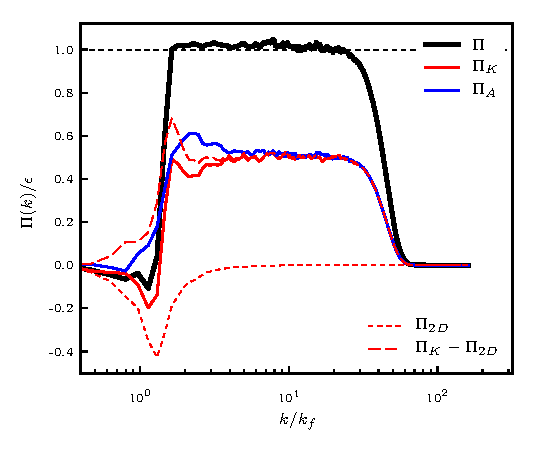
\includegraphics[angle=0]{./fig2.eps}}
 \caption{Spectral energy fluxes from run 1, normalised by the time averaged total energy dissipation $ \epsilon $.  }
 \label{F1}
 \end{figure}

Looking closer to Fig.~\ref{F1} we see that the kinetic energy flux, $ \Pi_K $, attains negative values at wave numbers around $ k_f $, which is a sign of an inverse energy cascade, although this is obviously very weak. A decomposition of  $ \Pi_K $ in the 2D part, containing contributions from interactions only involving $ {\bf u}_r $ and a remaining part, reveals that the 2D part (lower dashed red curve) is negative and thus produces an inverse energy cascade  while the remaining part (upper dashed red curve) is positive. The two contributions almost cancel each other at wave numbers close to $ k_f $. This is similar as seen in Fig.~\ref{Flux} from the GCM, although the inverse energy cascade is very weak in run 1.

\begin{figure}[h]
\centerline{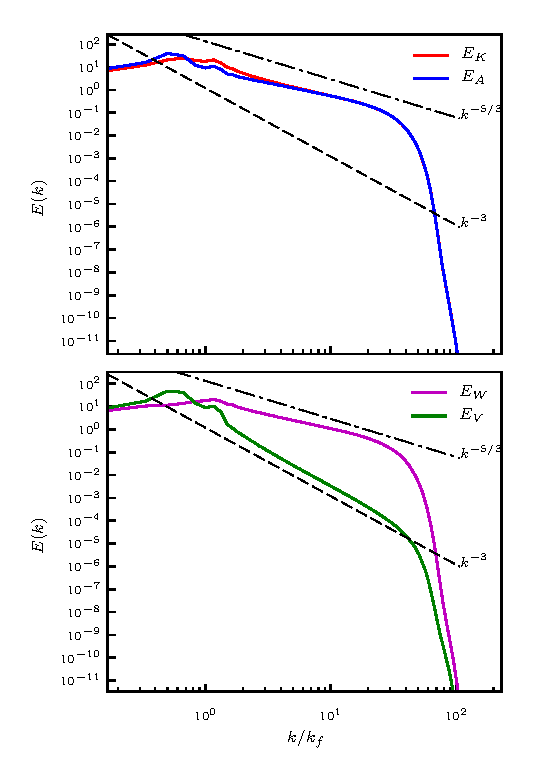
\includegraphics[angle=0,width=8.5cm]{./fig3.eps}}
 \caption{ Energy spectra from run 1. Upper plot is showing KE and APE spectra, while the lower plot is showing wave and vortical energy spectra. }
 \label{S1}
 \end{figure}


 In Fig.~\ref{S1} we see  time averaged energy spectra from run 1. The upper plot is
 showing the KE spectrum, $ E_K $,  and the APE spectrum, $ E_A$, while the lower plot
 is showing wave energy and the vortical energy spectra, $ E_W $ and $ E_V$.  In the
 forward cascade range, $ E_K $ and $ E_A $ are slightly more shallow than $ k^{-5/3} $,
 as is $ E_W $.  As can be seen from the upper plot, KE and APE are equipartioned at
 large wave numbers. Again, this is a characteristic feature of gravity waves. In the
 lower plot we see that $ E_V $  falls of approximately as $ k^{-3} $. Thus, at high
 wave numbers the wave field is totally dominant. At very low wave numbers, however, $
 E_V $ is slightly larger than $ E_W $, due to a slow build  up of vortical energy at
 large scales. { As we will argue in the following the approximate $ k^{-3} $-range of
 the vortical spectrum may be interpreted as an enstrophy or potential enstrophy cascade
 range of the same type as is found in 2D turbulence \citep{Kraichnan1967, Kraichnan1971}.}

{ It is not entirely clear why the wave energy spectrum is more shallow than $ k^{-5/3}
$ in run 1. One hypothesis would be that this can be explained by the so called
"bottleneck effect". Energy has a tendency to build up in the high wave number end of
the spectrum and this tendency becomes stronger with a higher degree of the diffusion
operator \citep{Haugen2004}. We have explored this hypothesis by carrying out a series
of simulations in which the only difference is the order of the diffusion operator. In
Fig.~\ref{Comp1} we see a plot of the compensated wave energy spectrum from three such
simulations,  using $ \Delta^{4} $ (run 1), another using $ \Delta^{2} $ and a third
using the Navier-Stokes diffusion operator $ \Delta $. Indeed, $ E_W $ drops a little
bit when we use $ \Delta^2 $ instead of $ \Delta^{4} $ and when we use $ \Delta $ we
obtain a pretty clean $ k^{-5/3} $-range, although it is limited. However, in this case
we also observed a clear decrease of the energy flux in the same range, which makes it
questionable if the deviation from $ k^{-5/3} $ entirely can be explained as a
bottleneck effect.  Another hypothesis is that  deviations from $ k^{-5/3} $ can be
generated as a consequence of the type of nonlinear interactions which are involved,
which in turn may be dependent on the type of forcing which is used. To explore this
hypothesis we carried out run 2, which is similar to run 1 in everything except in the
forcing scheme. While run  1 is primarily forced in  wave modes, run 2 is primarily
forced in vortical modes. In Fig.~\ref{Flux2} we see the energy fluxes from run 1 and
run 2 decomposed into the four contributions given in equation (\ref{Decomposition}). In
both runs $ \Pi_{VWW} $ is dominant. This flux is produced by triad interactions between
one vortical mode and two wave modes. However, in run 1 $  \Pi_{WWW} $ also makes an
important contribution, especially at high wave numbers, while $ \Pi_{VVW} $ is close to
zero. In run 2,  on the other hand,  $ \Pi_{VVW} $ makes an important contribution while
$ \Pi_{WWW} $ is close to zero. In both runs, $ \Pi_{VVV} $ is negative, which means
that triad interactions including three vortical modes produce an inverse cascade, as
expected.  In the left plot of Fig.~\ref{C2} we  see compensated wave energy spectra from
run 1 and run 2. Comparing the two runs we see that there is a range where the
compensated spectrum is flat in run 2, which means that we have a pretty clean $
k^{-5/3} $ range, while the compensated spectrum of run 1 is exhibiting a ``bump'' in the
high wave number range.  In all likelihood the difference is associated with the
difference in the type of triad interactions that is producing the cascade. In run 2,
VWW-interactions are totally dominant at high wave number, while WWW-interactions also
make important contributions in run 1. It is likely that the ``bump'' is associated with
these WWW-interactions. In the right plot of Fig.~\ref{C2} we see the uncompensated
vortical energy spectra from run 1 and run 2. Here, there is an even larger difference.
The vortical spectrum from run 2 is much more shallow, close to $ k^{-5/3} $,  than the
$ k^{-3} $ vortical spectrum from run 2. The difference between the two spectra is
associated with a difference in potential energy flux. In Fig.~\ref{EF1} we see the
potential energy flux, $ \Pi_q $,  from run 1 (left) and run 2 (right). In run 1,  there
is a range  which is reminiscent of a constant flux range, although there is slow
increase of  $ \Pi_q $. In run 2, on the other hand, there is a rapid increase of $
\Pi_q $ at high wave numbers where it reaches value which is eighty times larger than in
run 1. These results suggest that the $ k^{-3} $-spectrum of run 1 can be interpreted as
an enstrophy or potential enstrophy inertial range spectrum, although $ \Pi_q $ is not
perfectly constant. Whether or not such a range is obtained should mainly depend on $ Ro
$ and $ Fr $. In the quasigeostrophic limit, $ Ro \rightarrow 0 \, , Fr \rightarrow 0 $,
such a range should always be obtained, since potential enstrophy is an inviscidly
conserved quantity in this limit. At finite $ Ro $ and $ Fr $, different initial
conditions or different forcing mechanisms, may evidently also be important as to
whether such a range is obtained.}

\begin{figure}[h]
\centerline{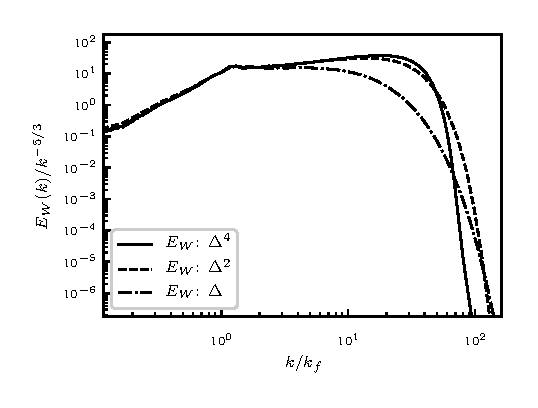
\includegraphics[angle=0]{./fig4.eps}}
 \caption{Wave energy spectra from simulations with different degrees of the diffusion operator.  }
 \label{Comp1}
 \end{figure}

 \begin{figure}[h]
\centerline{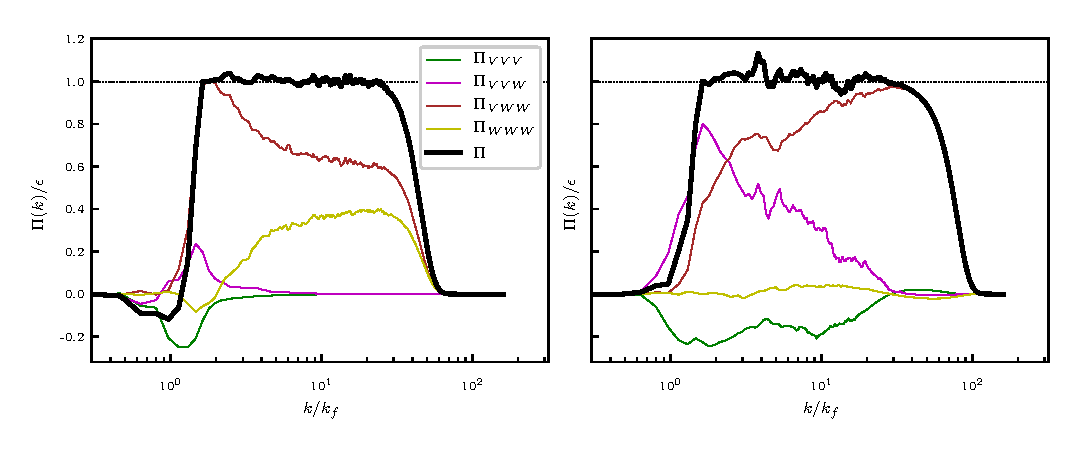
\includegraphics[angle=0]{./fig5.eps}}
 \caption{Energy fluxes from run 1 (left) and run 2 (right) decomposed into different contributions. }
 \label{Flux2}
 \end{figure}

  \begin{figure}[h]
\centerline{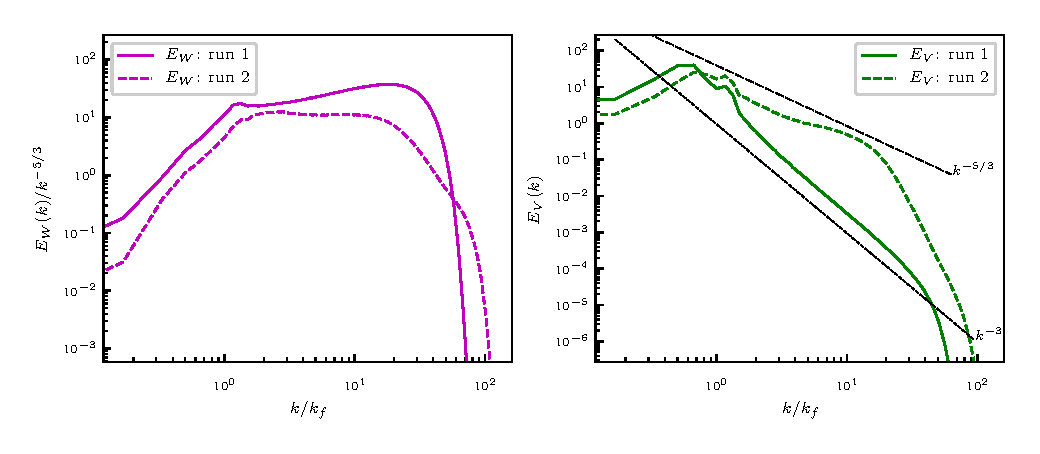
\includegraphics[angle=0]{./fig6.eps}}
 \caption{Compensated wave energy spectra (left) and uncompensated vortical spectra (right) from run 1 and run 2. }
 \label{C2}
 \end{figure}



\begin{figure}[h]
\centerline{\includegraphics[angle=0]{./fig7.eps}}
 \caption{Potential enstrophy flux from run 1 (left) and run 2 (right). }
 \label{EF1}
  \end{figure}



\begin{figure}[h]
\centerline{\includegraphics[angle=0]{./fig8.pdf}}
\caption{Divergence field from a simulation of the shallow water equations (left) and from run 1 of the toy model (right). }
\label{Shocks}
 \end{figure}

\begin{figure}[h]
\centerline{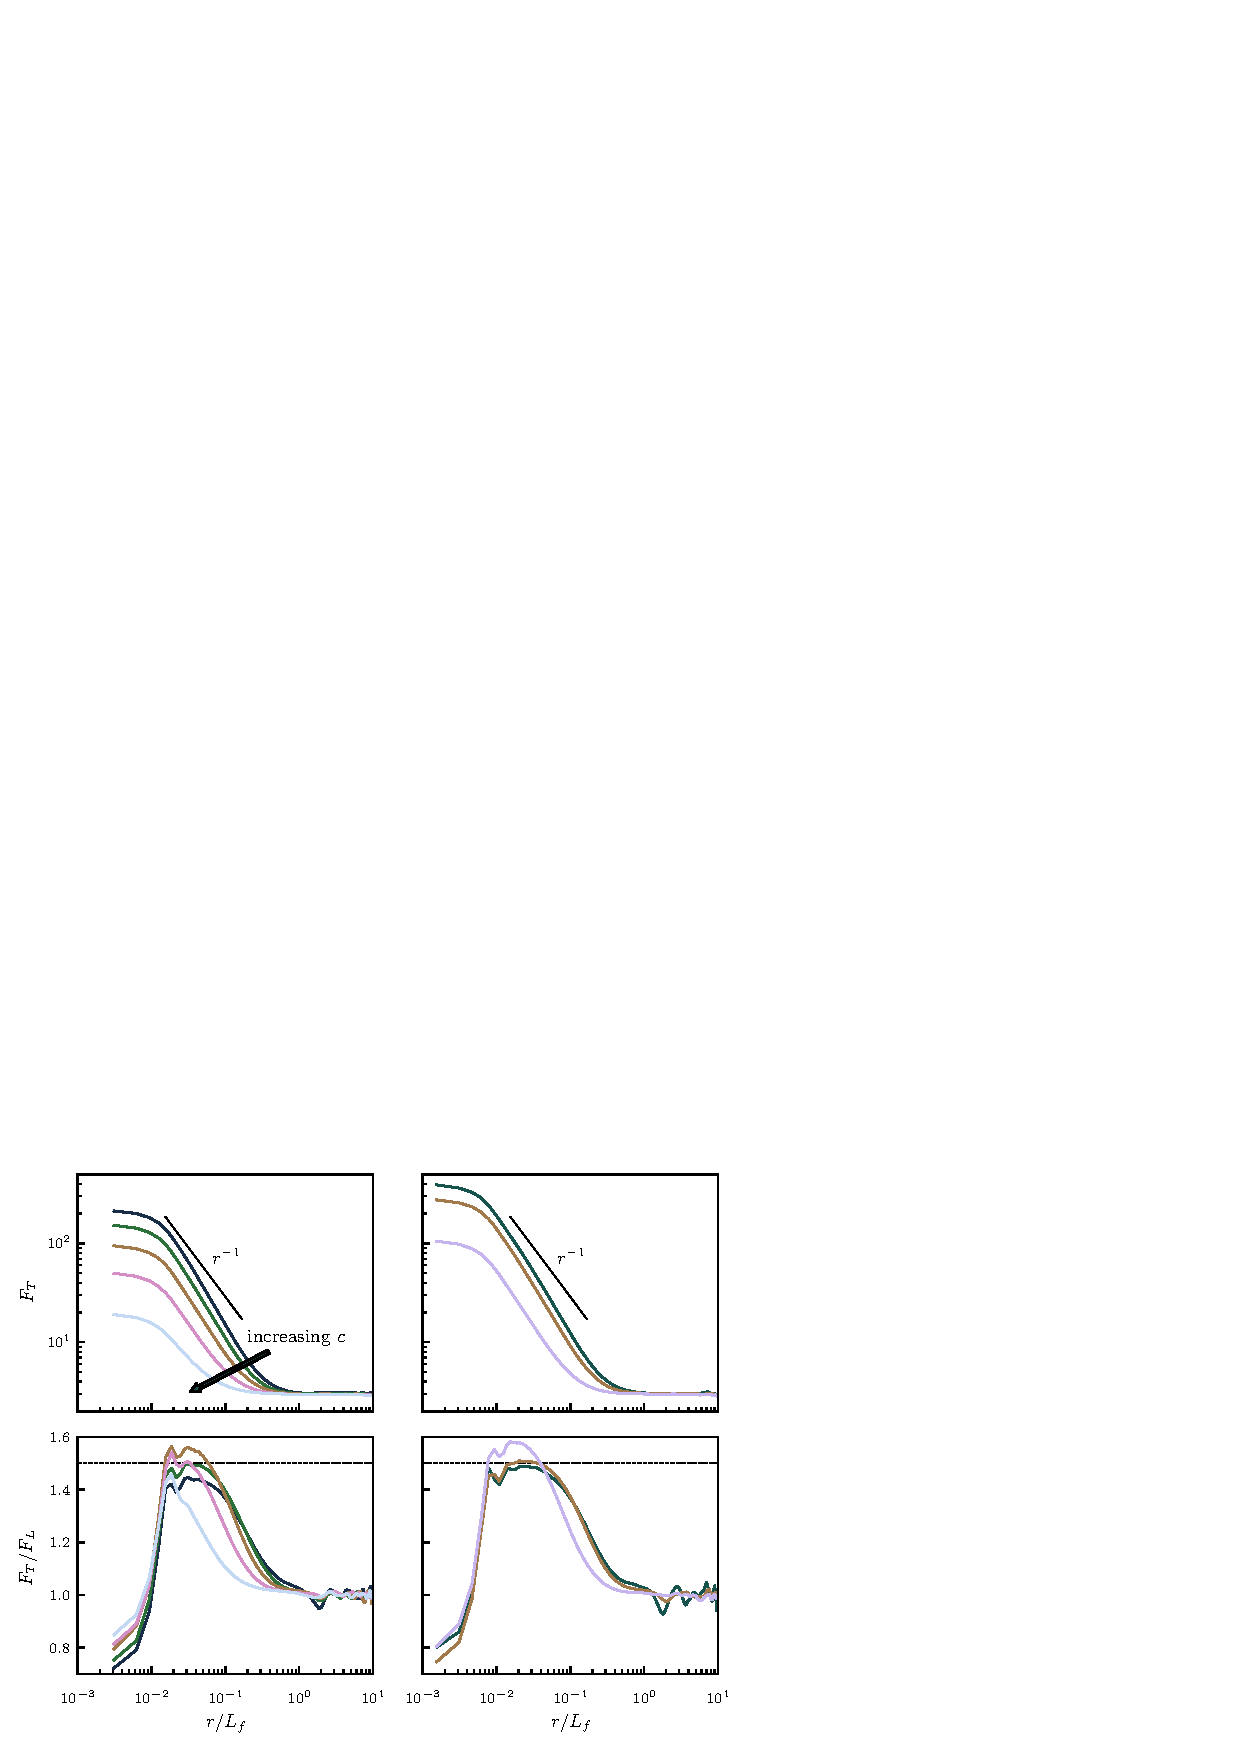
\includegraphics[angle=0]{./fig9.pdf}}
\caption{Potential vorticity field (left) and wave field (right) from the end state of run 1.}
\label{Vis1}
\end{figure}


 We now turn to the question regarding possible shock generation in the toy model.  We have found that the most reliable method of detecting shocks visually is to plot the divergence field. Shocks are displayed as thin lines of high amplitude negative divergence in such plots. The higher the resolution is, the thinner are the lines, since the width of the shocks scales with the smallest length scale that is resolved if there is sufficient viscosity to diffuse the shocks over this scale.
That the divergence is negative along the shocks  can be understood from the fact that the velocity component perpendicular to the shock has a negative jump in the direction of shock propagation.  Consider a shock which is parallel to the $ y $-axis and is traveling in the positive $ x $-direction. The velocity component in the $ x $-direction, $ u $, is positive on both sides of the shock, but is  smaller behind than in front of the shock. This jump in $ u $ is seen as a high amplitude negative value of $ \partial_x u $, which is the divergence. In Fig.~\ref{Shocks} we have plotted the divergence field from a simulation of the shallow water equations (to the left) together with the divergence field from run 1 (to the right).
The simulation of the shallow water equations has a similar set up as run 1.
{ Comparing the two plots one should not compare the absolute values of divergence, which scale differently in the two simulations, but  the pattern. In the left plot, long bands of high amplitude negative divergence are displayed against a background of almost uniform low amplitude divergence. These bands are signatures of shocks. In the right plot, on the other hand, we see tightly packed alternating bands of high amplitude negative and positive divergence. These bands are signatures of a continuous wave field.}
We can quite safely conclude that the toy model does not produce any shocks, just as we argued in the previous section.

In Fig.~\ref{Vis1} we see the potential vorticity field (left plot) and the wave field (right plot) corresponding to one of the wave field modes, namely $ \widehat{a_1} $. There is a huge difference in the visual appearance of the two fields. The vortical field develops structures at much larger length scales and with very different shapes than the elongated fronts of the wave field. A blow up display the wave structures in more detail.



We now turn our attention to run 3, where the only change we did in comparison to run 1, was to force in $ k_f = 30 $ instead of $ k_f = 6 $. The idea is that the inverse energy cascade can develop over a larger span of wave numbers if we use a larger $ k_f $ and may therefore become stronger.  In Fig.~\ref{F2} we see the spectral energy fluxes normalised by the total energy dissipation from run 3.  In this plot we have also included the cumulative spectral APE-KE conversion, $ C_{cum} $,  defined in (\ref{Cum}). In the forward  cascade range the fluxes are similar to what we saw in run 1, with $ \Pi_K = \Pi_A $ at high wave numbers --  a sign of gravity waves with equipartition between $ E_K $ and $ E_A $. At wave numbers $ k < k_f $ the total flux (black curve) is clearly negative which means that a substantial amount of energy is transferred upscale. This upscale cascade
 is produced by interactions involving only the rotational component  of the velocity field. The lower red dashed curve, $ \Pi_{2D} $, is the negative flux produced by these interactions and the upper dashed red curve is the positive flux produced by the remaining type of interactions, also involving the divergent component.  The cumulative spectral conversion, $ C_{cum} $ (green curve), displays a strong decrease around the forcing wave number. The decrease of $ C_{cum} $ is equal to the APE-KE conversion in the corresponding wave number range and is approximately matched by a corresponding increase of $ \Pi_K $ in the same wave number range. This is similar to what is seen in Fig.~\ref{Flux} showing energy fluxes from a GCM. An interesting feature of $ C_{cum} $ is the strong positive gradient seen at a lower wave number than $ k_f $. That the gradient is positive means that there is conversion from KE to APE at the corresponding wave number. The energy which is converted  from KE to APE at this low wave number starts to cascade downscale which is seen from the positive APE flux at  $ k < k_f $.  At very low wave numbers, $ k \rightarrow 0 $, $ C_{cum} $ approaches the total APE-KE conversion.



\begin{figure}[h]
\centerline{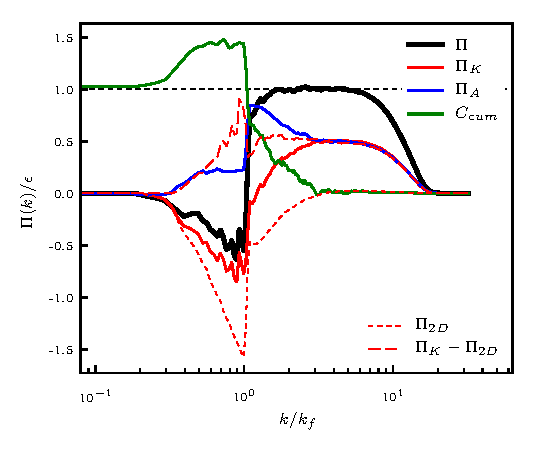
\includegraphics[angle=0]{./fig10.eps}}
 \caption{Spectral energy fluxes from run 3, normalised by the time averaged total energy dissipation $ \epsilon $. }
 \label{F2}
 \end{figure}



 \begin{figure}[h]
\centerline{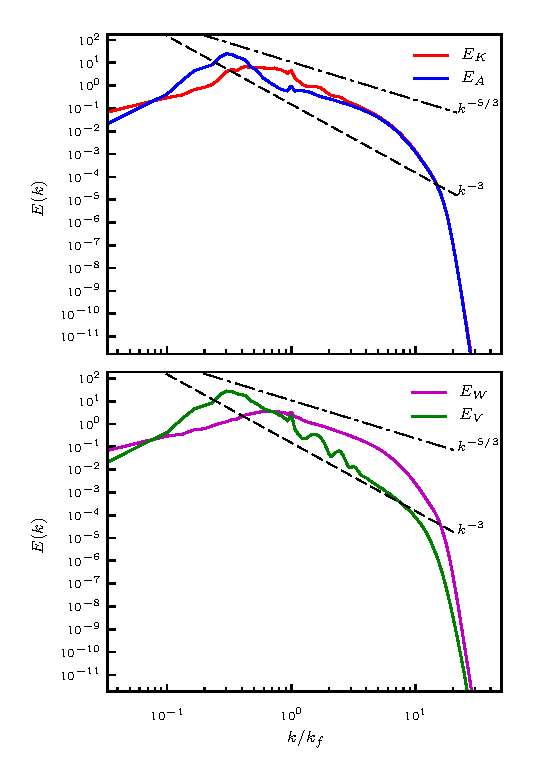
\includegraphics[angle=0,width=8.5cm]{./fig11.eps}}
 \caption{ Time averaged energy spectra from run 3. Upper plot is showing KE and APE spectra, while the lower plot is showing wave and vortical energy spectra. Averaging was made over the intervall $ t/\tau \in [756 \; 1224] $.}
 \label{S2}
 \end{figure}

 \begin{figure}[h]
 \centerline{\includegraphics[angle=0]{./fig12.eps}}
\caption{Potential vorticity field (left) and wave field (right) from the end state of run 3.}
 \label{Vis2}
 \end{figure}

\begin{figure}[h]
\centerline{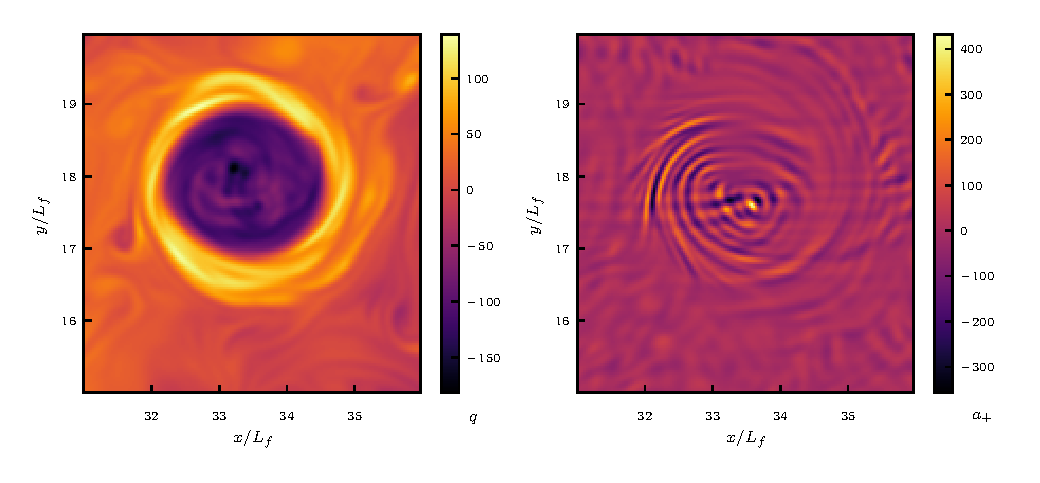
\includegraphics[angle=0]{./fig13.eps}}
\caption{Blow up of the potential vorticity field (left) of a strong anticyclonic vortex and the corresponding wave field (right). }
\label{Vis3}
\end{figure}




In Fig.~\ref{S2} we see the time averaged energy spectra averaged over a time
interval during the end of run 3.  In the upper plot we see that $ E_K $ and $ E_A $ {
are equal or equipartioned} at high wave numbers, just as in run 1. At low wave
numbers, there is a stronger build up of $ E_A $ than $ E_K $, despite the fact that
the inverse energy cascade is restricted to KE. This can be explained by the KE-APE
conversion at small wave numbers that we just discussed.  In the lower plot we see that
$ E_W $ is falling off very close to $ k^{-5/3} $ in a limited range at wave numbers
larger than $ k_f $. At very high wave numbers  $ E_W $  is decreasing faster than in
run 2 and no bottleneck is observed. This may be due to the fact that the effective
diffusion coefficient is larger in run 3 as compared to run 1, since the total
dissipation is lower while we use the same numerical value of $ \nu_4 $.  Just as in
run 1, $ E_{V} $ has an approximate $ k^{-3} $-dependence in a broad range. However,
in Fig.~\ref{S2} we see some wiggles of $ E_W $ which were not present in run 1,
neither  in earlier stages of run 3, but only in the late stage. Taking a closer look
at the upper plot, we can see that these wiggles are also present in $ E_K $. It may be
suggested that these wiggles somehow are produced by the forcing. However, since they
were neither observed in run 1 nor in the earlier stages of run 3, we find it more
likely that there is another explanation. { As we saw in run 2, the vortical spectrum
may also display a more shallow dependence, close to $ k^{-5/3} $, if forcing is
applied in vortical modes. It may be the case that the late stage of run 3 has reached
a state in which the $ k^{-3} $ vortical spectrum is unstable and subsequently will be
replaced by a more shallow spectrum. }

The  potential enstrophy flux, $ \Pi_q $,  in run 3 had a very similar appearance as in run 1, why we don't show this plot.



In Fig.~\ref{Vis2} we show visualisations of the vortical field (left plot) and the wave field (right plot) from the end state of run 3. In the left plot we see that a multitude of coherent vortices has emerged in the vortical field. There is a strong dominance of anti-cyclonic vortices, displayed as dark,  almost circular,  disks of negative $ q $. An interesting feature of these vortices is that they are surrounded by  thin filaments of positive $ q $, displayed in yellow. The strong dominance of anti-cyclonic vortices has also been observed in shallow water  simulations by several investigators  \citep{Cushman1990, Arai1994, Polvani1994, Cho1996} and there have been many attempts to explain the phenomenon. An excellent review on the matter is given by \citet{Graves2006}, together with a plausible explanation. According to these authors, anti-cyclonic dominance is not only a feature of the shallow water equations but is also seen in natural flows in which the influence of boundaries is secondary. In the right plot we see that the wave field in run 3 displays much smaller structures than the vortical field, just as in run 1.  As can be seen from the blow up of the wave field inserted in the right plot, vortices are strong centres of high wave activity and the wave field within a vortex displays patterns that follow the organisation of the vortex filaments.  In Fig.~\ref{Vis3} we see a blow up of the potential vorticity field (left) of a strong anticyclonic vortex and the corresponding wave field in the same vortex (right). The high level of wave activity within the vortex suggests that there is a high level of energy dissipation in the vortex.  It is one of the most fascinating mysteries of fluid dynamics how  long live vortices may be sustained in the presence of dissipation.

 \section{Conclusions}

Comparing the spectral energy fluxes from a full GCM shown in Fig.~\ref{Flux} with the corresponding fluxes in Fig.~\ref{F2} from run 3 of the toy model we see that there is a striking similarity. A considerable amount of APE which is forced at large scales is converted into KE. A part of the KE is going into a downscale cascade at $ k > k_f $, while the other part, which is of the same order of magnitude, is going into an upscale cascade at $ k < k_f $. The upscale cascade is restricted to KE and is produced by interactions only involving the rotational component of the velocity field. The downscale energy cascade, on the other hand, is a cascade of both APE and KE. Here we also see an important difference. In the toy model there is perfect equipartition between KE and APE at high wave numbers and also between the fluxes $ \Pi_K $ and $ \Pi_A $. In the GCM, on the other hand, $ \Pi_K > \Pi_A $ at corresponding wave numbers. Clearly, the downscale energy cascade in the GCM is not a clean wave energy cascade with equipartition between KE and APE. \citet{Callies-Ferrari-Buhler:2014} have suggested that the mesoscale $ k^{-5/3} $ spectrum is produced by inertia-gravity waves with frequencies that are close to $ f $. For such waves, $ E_K > E_A $. However, the kinetic energy content in the rotational component of the velocity field is necessarily smaller than in the divergent component, and that is at odds with observational evidence \citep{Lindborg:2015, QiangLi2017}.  There is also numerical evidence \citep{Deusebio-Vallgren-Lindborg:2013, Asselin2017} suggesting that the forward energy mesoscale energy cascade cannot be described as a cascade of waves at high wave numbers, although it may start as a wave cascade at low wave numbers. In any case, as we pointed out earlier, the forward energy cascade in the GCM cannot be produced by inertia-gravity waves with frequencies close to $ f $, since it would require much finer resolution in the vertical to simulate such motions. Neither can it be fully accounted for by stratified turbulence as suggested by \citet{Lindborg2006}, since that would also require much finer resolution. In the toy model simulation, on the other hand, we have been able to simulate a downscale energy cascade using only a single level. All nonlinear interactions that are present in the toy-model are also present in the dynamical equations of a full GCM, at each level. Moreover, in the GCM both $ E_A $   and $ E_K $ can be expressed as quadratic quantities to lowest order and the  sum of $ E_A $ and $ E_K $ is approximately conserved. Therefore, it seems likely that the toy model catches the essential cascade dynamics of the GCM. An important difference is, of course, that  inertia-gravity waves in the full GCM, as well as in nature, are three-dimensional, anisotropic and much more dispersive than in the toy model.

{The toy model is a tool by which energy and enstrophy cascades can be studied from the point of view of turbulence theory. Since the expressions for $ E_A $  and $ E_K $ are quadratic, the dynamics can be investigated by means of triadic interactions in Fourier space, just as 2D turbulence.  As we have shown in this study different types of interactions between vortical and wave modes may result in different cascade pictures. What types of interactions that are activated is not only dependent on $ Ro $ and $ Fr $ but also on the type of forcing which is used. Different types of forcing may lead to different types of cascades. If forcing is primarily applied in  wave modes, as in run 1, the vortical energy spectrum displays a $ k^{-3} $-range associated with a positive enstrophy flux which is limited, although not perfectly constant.  On the other hand, if forcing is primarily applied in vortical modes, as in run 2, the vortical energy spectrum is much more shallow, close to $ k^{-5/3} $, and the potential enstrophy flux is much larger. Evidently, vortical energy may either display an enstrophy cascade range or an energy cascade range depending on what types of interaction are activated. In a future study we will investigate this further.
}

A limitation of this study is that we have carried out the simulations on an $ f $-plane without including the $ \beta $-effect. The $ \beta $-effect may easily be included in the model. Another possible continuation is to implement the model on a rotating sphere and compare the results with simulations of the shallow water equations which were carried out by \citet{Cho1996}. Since the toy model shows the same type of cyclonic/anticyclonic asymmetry as the shallow water equations it may also be used as a tool to further investigate this issue. A definite advantage in this context, is that the model does not produce any shocks.

Indeed,  the toy model is constructed to meet certain mathematical desiderata -- quadratic expression for total energy and absence of shocks -- rather than as a model of a physical system that can be set up in an experiment.  In vain, we have tried to derive the model by constructing a gedanken experiment of a physical system that  to lowest order would evolve in accordance with the model equations. Until such a derivation is presented, we have to be content in using it as nothing more, nothing less,  than a toy.

%\begin{figure}[h]
%\centerline{\includegraphics[angle=0]{./Fig12.eps}}
% \caption{Time averaged potential enstrophy flux from run 2, displayed in a log-log plot. The sign has been reversed in the low wave number range, where the flux is negative (dashed line), implying that potential enstrophy is going both upscale and downscale.  Averaging was made over the intervall $ t/\tau \in [756 \; 1224] $.}
 %\label{EF2}
 % \end{figure}


% If in two-column mode, this environment will change to single-column format so that long equations can be displayed.
% Use only when necessary.
%\begin{widetext}
%$$\mbox{put long equation here}$$
%\end{widetext}p

% Figures should be put into the text as floats.
% Use the graphics or graphicx packages (distributed with LaTeX2e).
% See the LaTeX Graphics Companion by Michel Goosens, Sebastian Rahtz, and Frank Mittelbach for examples.
%
% Here is an example of the general form of a figure:
% Fill in the caption in the braces of the \caption{} command.
% Put the label that you will use with \ref{} command in the braces of the \label{} command.
%

% Tables may be be put in the text as floats.
% Here is an example of the general form of a table:
% Fill in the caption in the braces of the \caption{} command. Put the label
% that you will use with \ref{} command in the braces of the \label{} command.
% Insert the column specifiers (l, r, c, d, etc.) in the empty braces of the
% \begin{tabular}{} command.
%
% \begin{table}
% \caption{\label{} }
% \begin{tabular}{}
% \end{tabular}
% \end{table}

% If you have acknowledgments, this puts in the proper section head.
\section*{Acknowledgments}
We thank  Pierre Augier  for interesting discussions and for helping us with the development of the code. Financial support from the Swedish Research Council (VR) is gratefully acknowledged. We thank two anonymous reviewers for useful comments and suggestions.
The simulations were performed on resources provided by the Swedish National Infrastructure for Computing (SNIC)  at  PDC.

% Create the reference section using BibTeX:


% \bibliography{references}

% \end{document}
%
% ****** End of file aiptemplate.tex ******
